\begin{frame}
  \frametitle{Porous Media: Current Approach}
  \begin{itemize}
  \item treated by the theory of homogenization
    \centerline{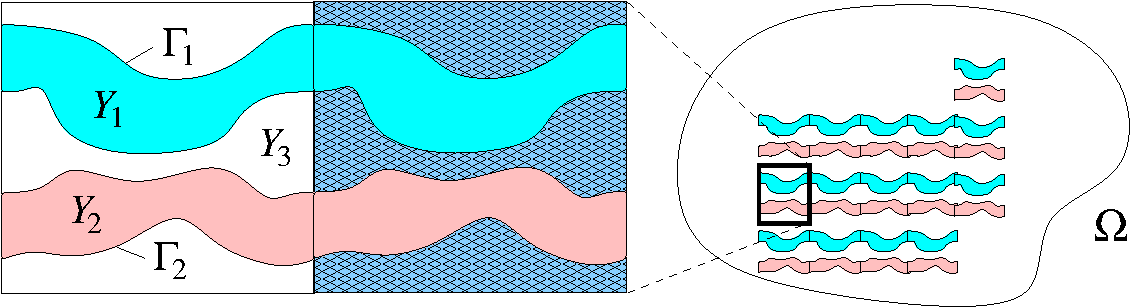
\includegraphics[width=0.6\linewidth]
      {\figDirHomPerfusion/fig_2porous_Y-domain-new-hsm}}
  \item modeling \emph{blood perfusion} in muscles, brain
  \item compact \emph{bone poromechanics}
  \item fading memory effects, \emph{stress recovery} at micro-level
  \end{itemize}
  \begin{center}
    \begin{minipage}[t]{0.6\linewidth}
      \scriptsize
      microstructure: two channels + porous matrix
      \begin{center}
        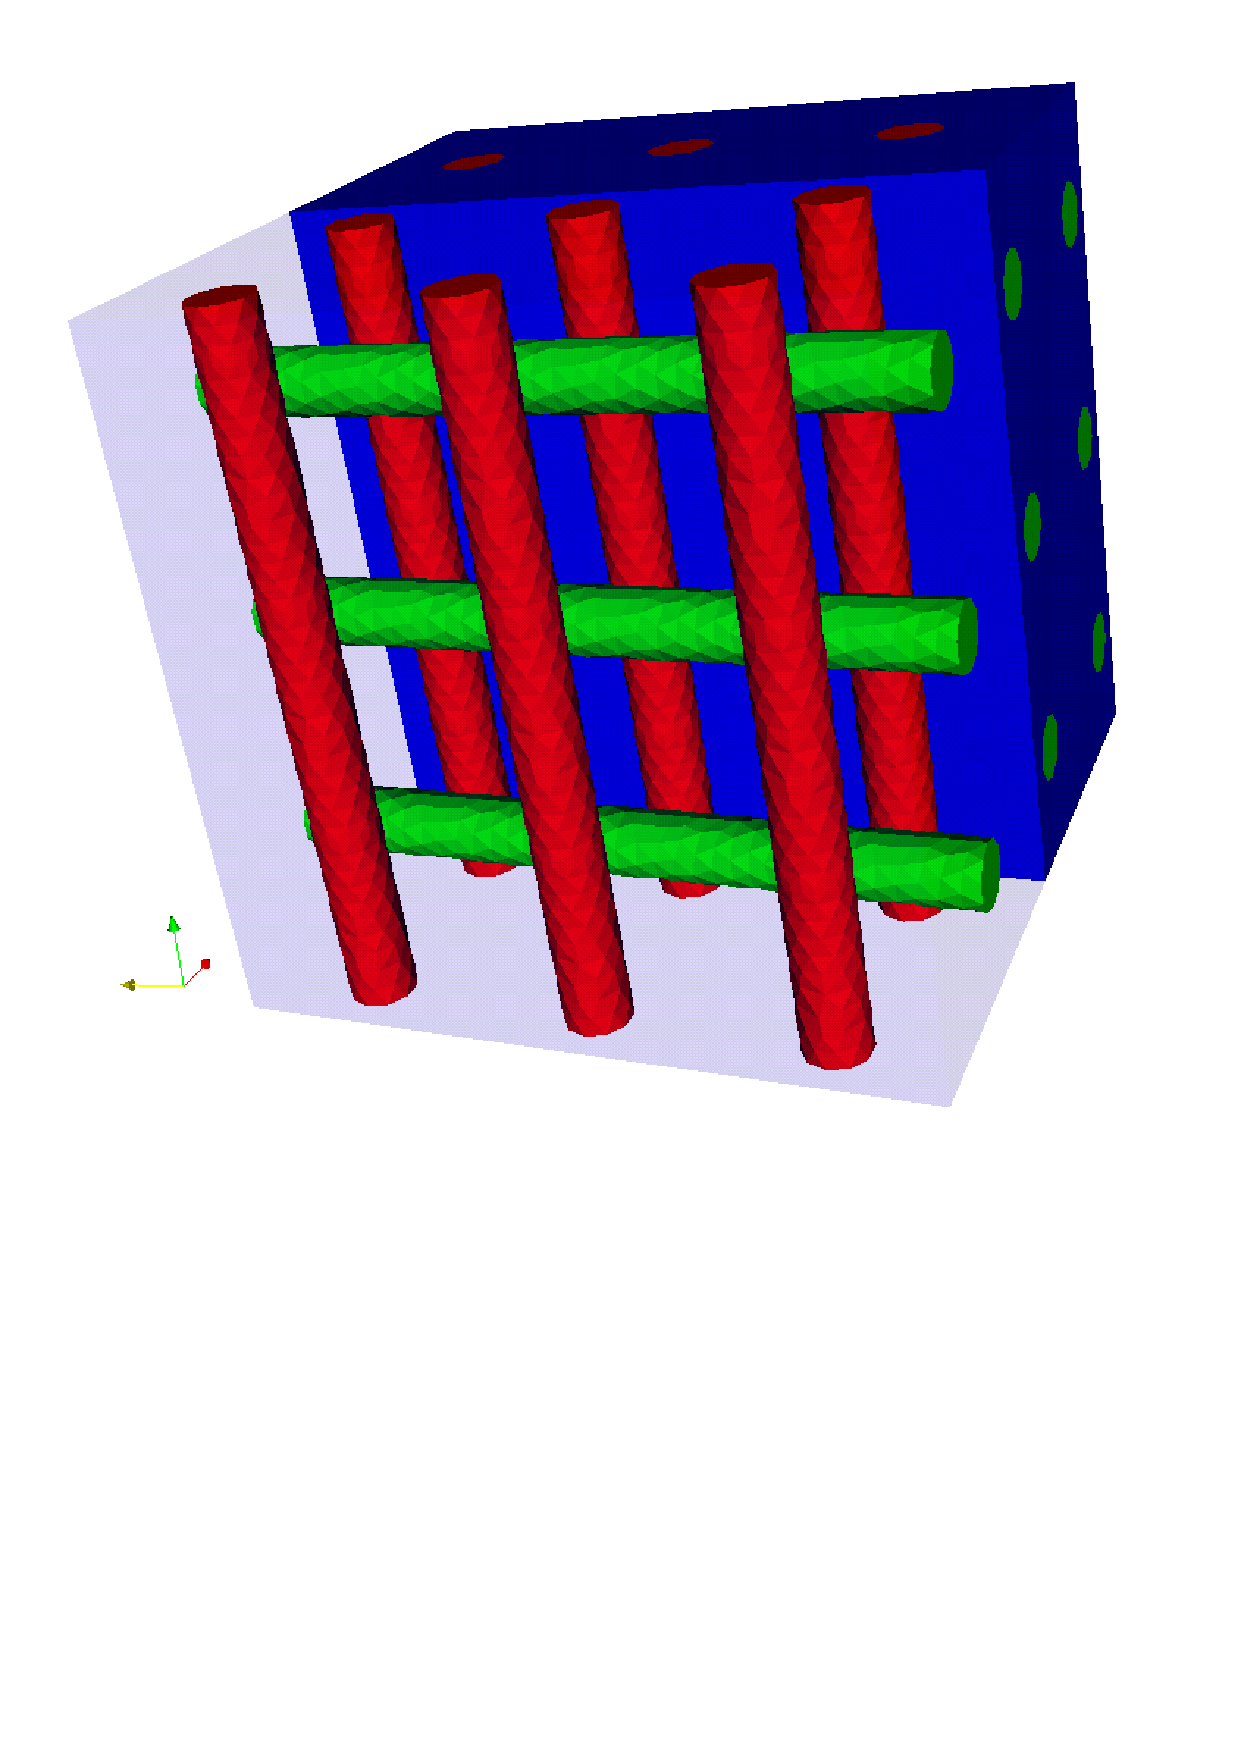
\includegraphics[width=0.5\linewidth]{\figDirHomPerfusion/micro_3d_M1}
        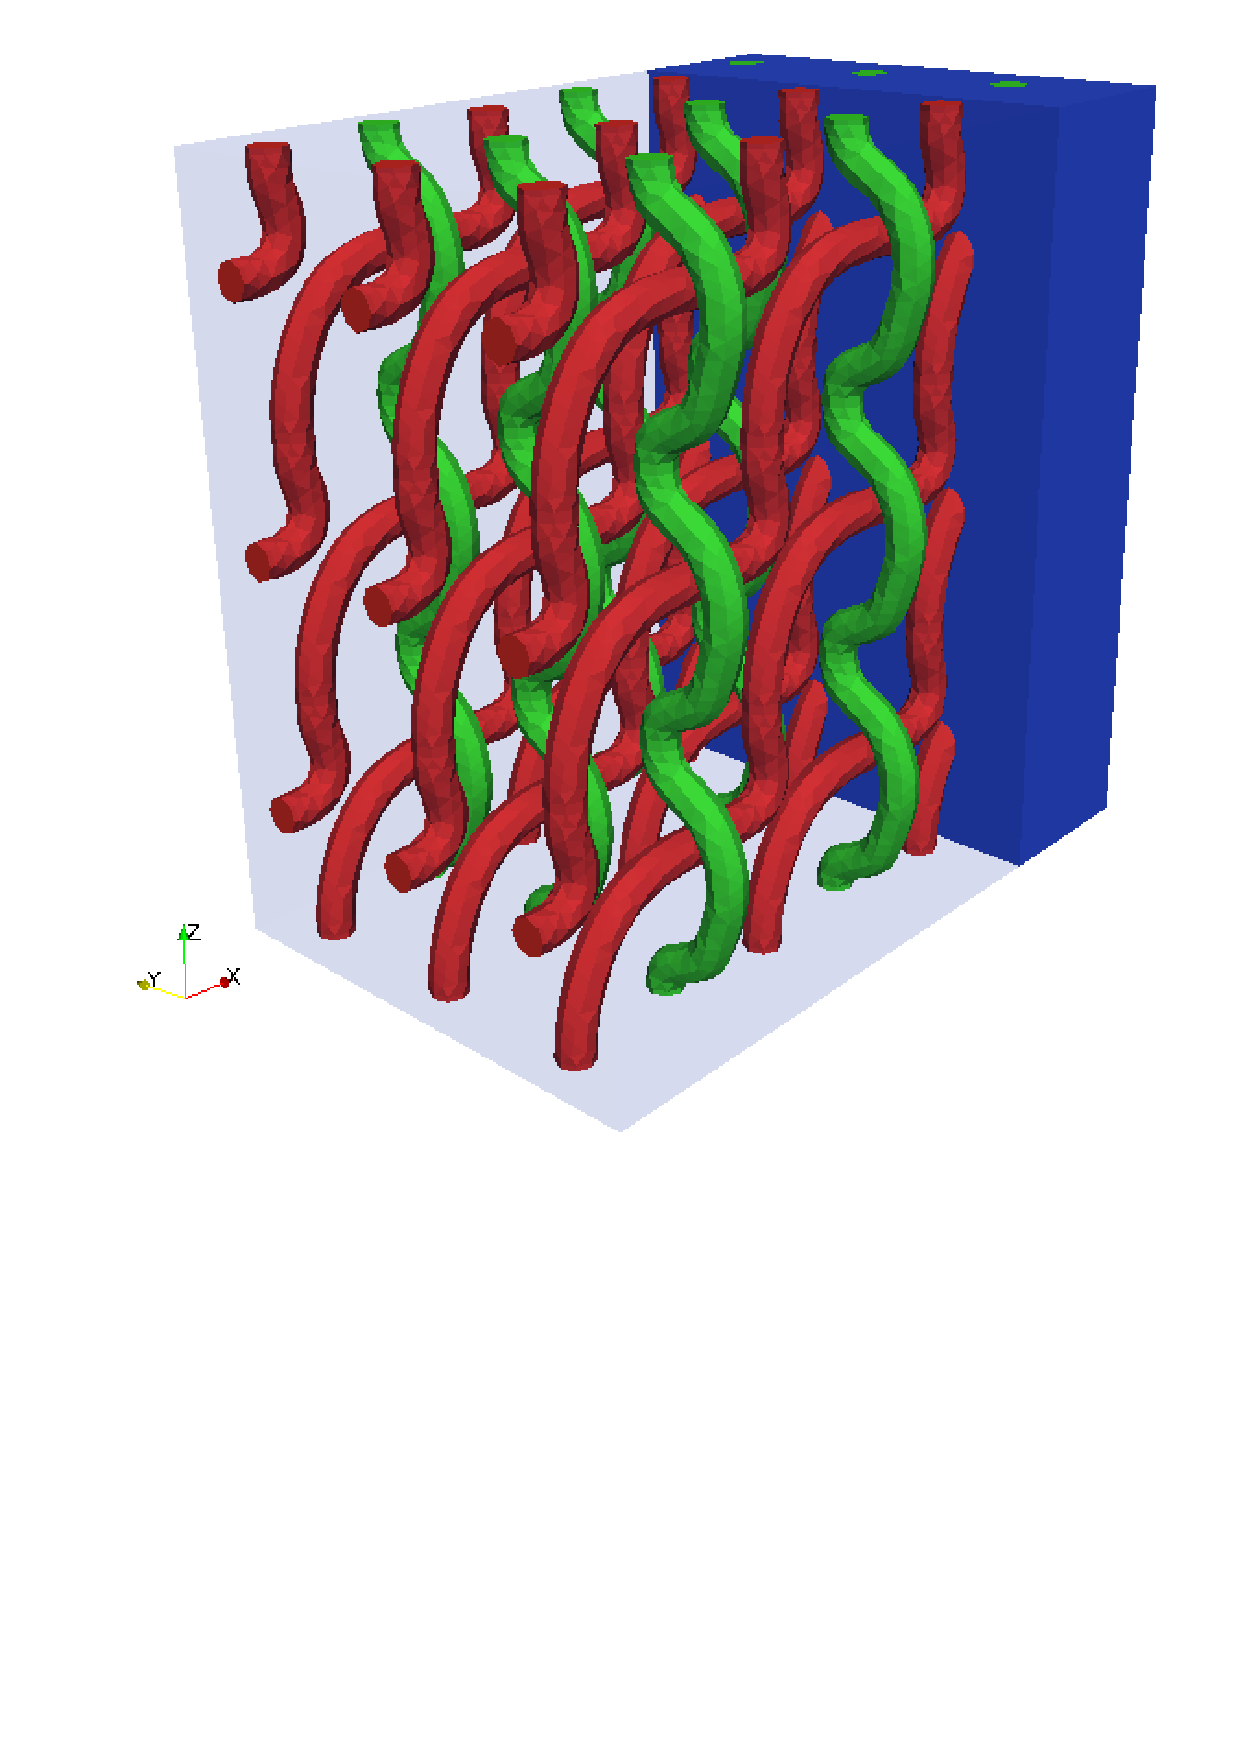
\includegraphics[width=0.5\linewidth]{\figDirHomPerfusion/micro_3d_M2}
      \end{center}
    \end{minipage}
    \hfill
    \begin{minipage}[t]{0.32\linewidth}
      \scriptsize
      microscopic corrector functions
      \begin{center}
        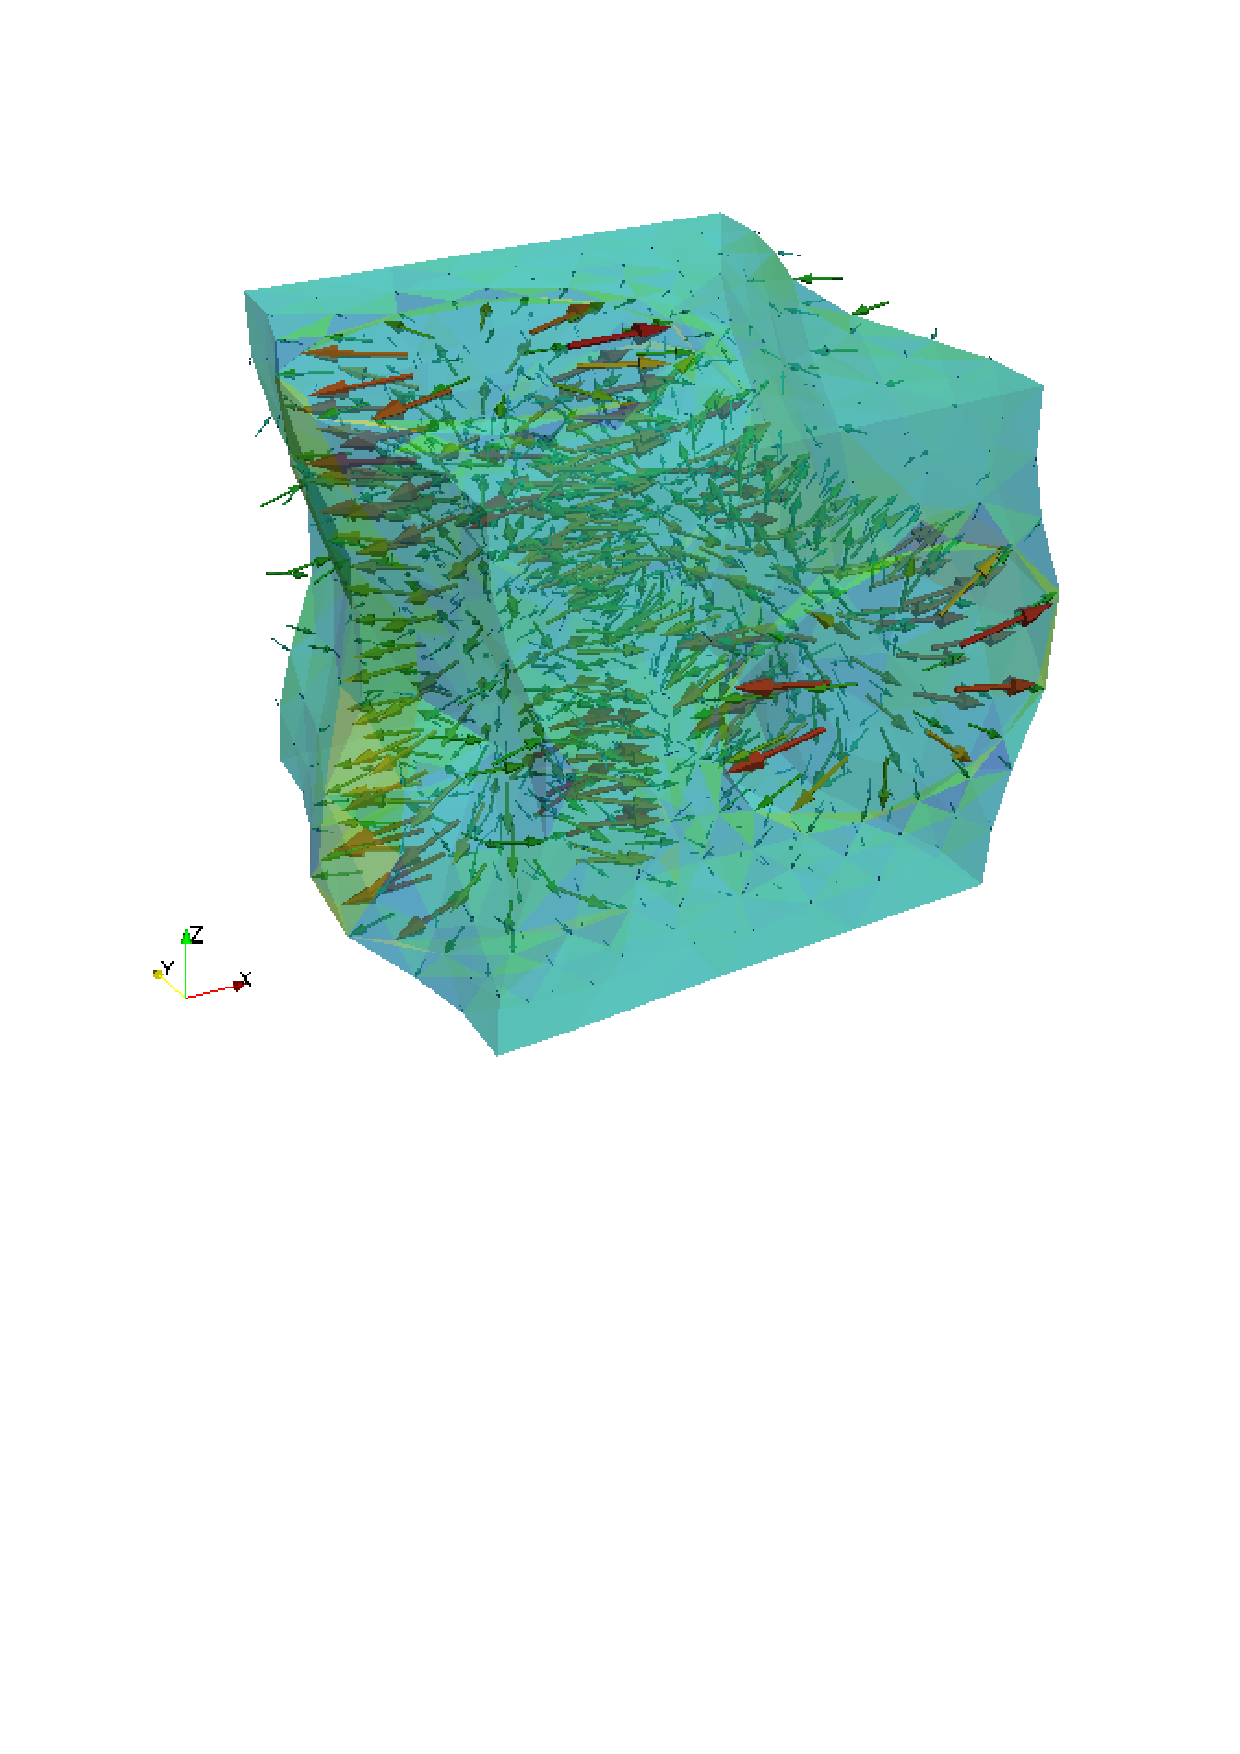
\includegraphics[width=0.5\linewidth]
        {\figDirHomPerfusion/steady_rs_00_u_M1_2}
        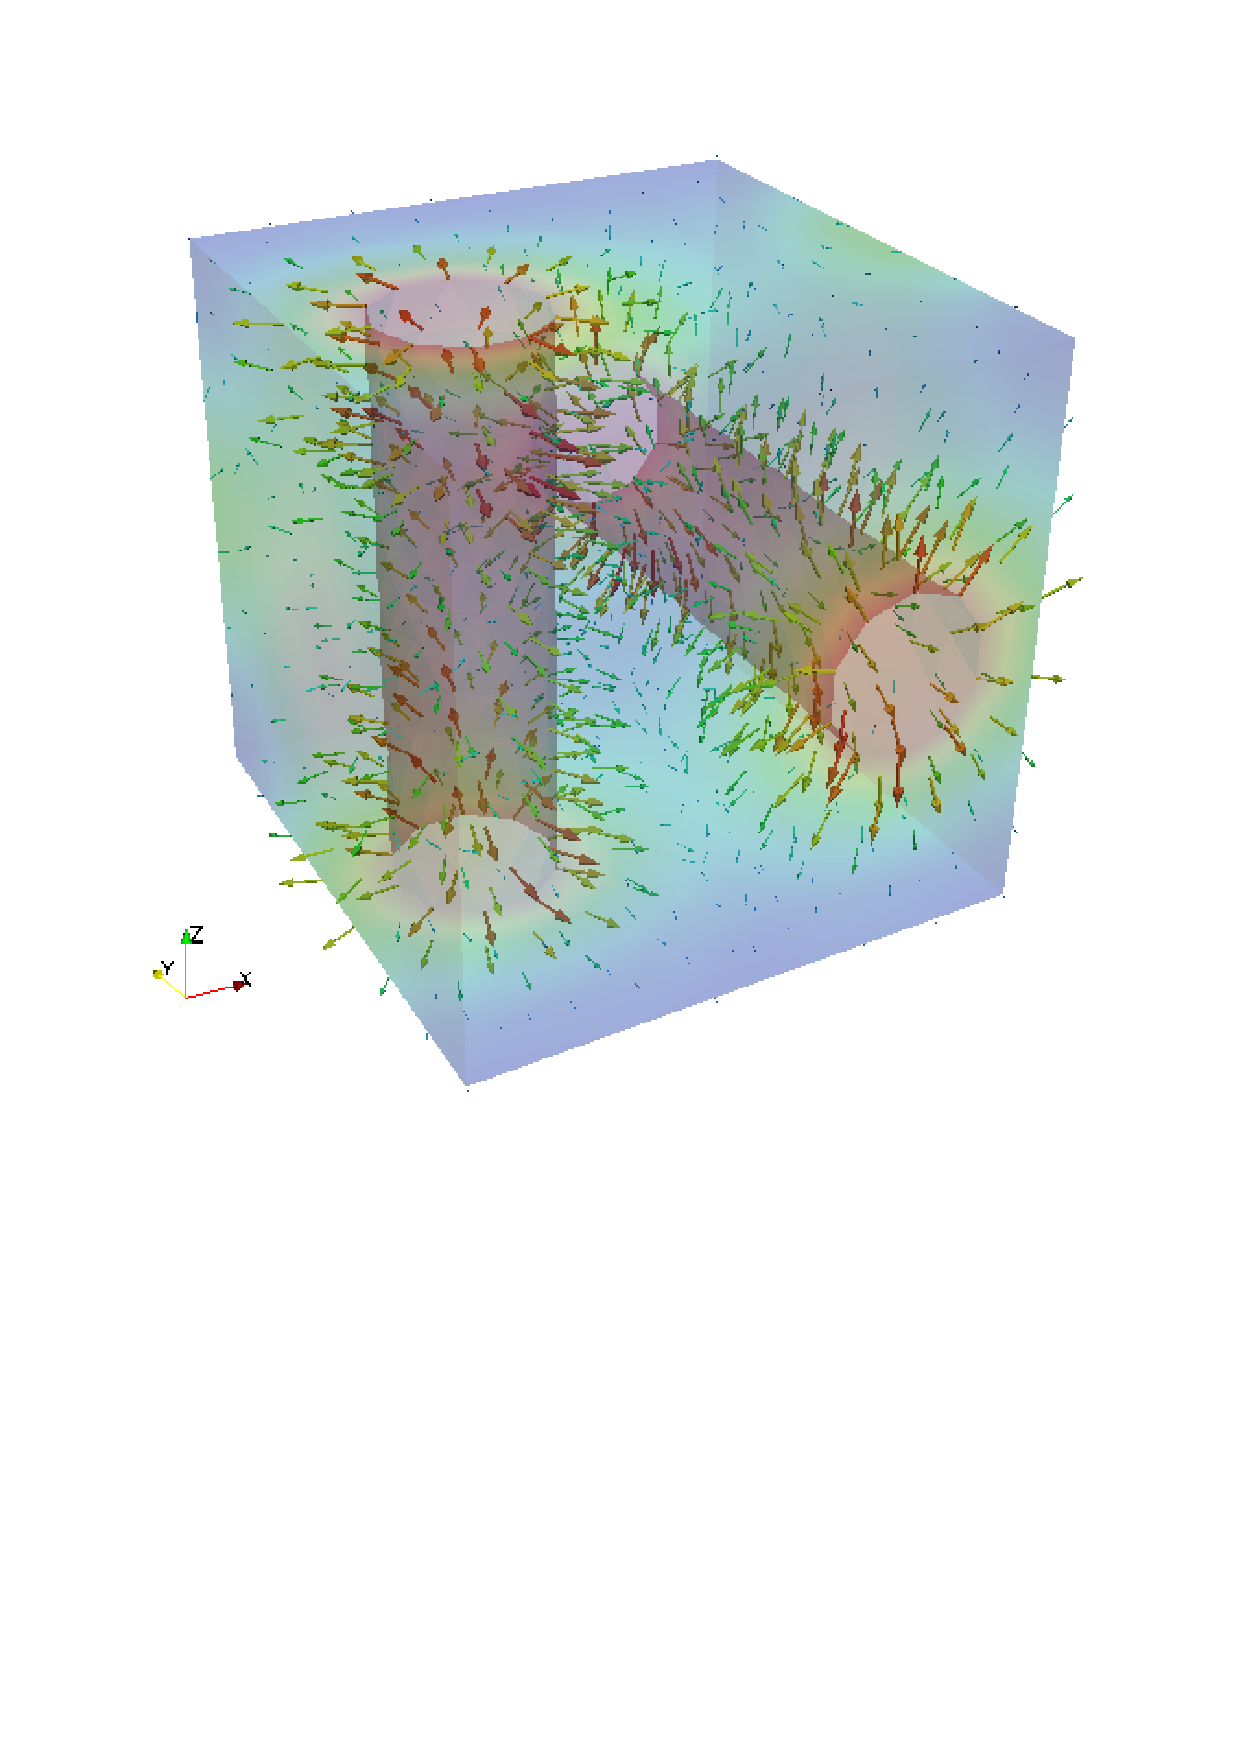
\includegraphics[width=0.5\linewidth]
        {\figDirHomPerfusion/steady_rs_00_p_M1_2} \\
        \vspace*{-10mm}
        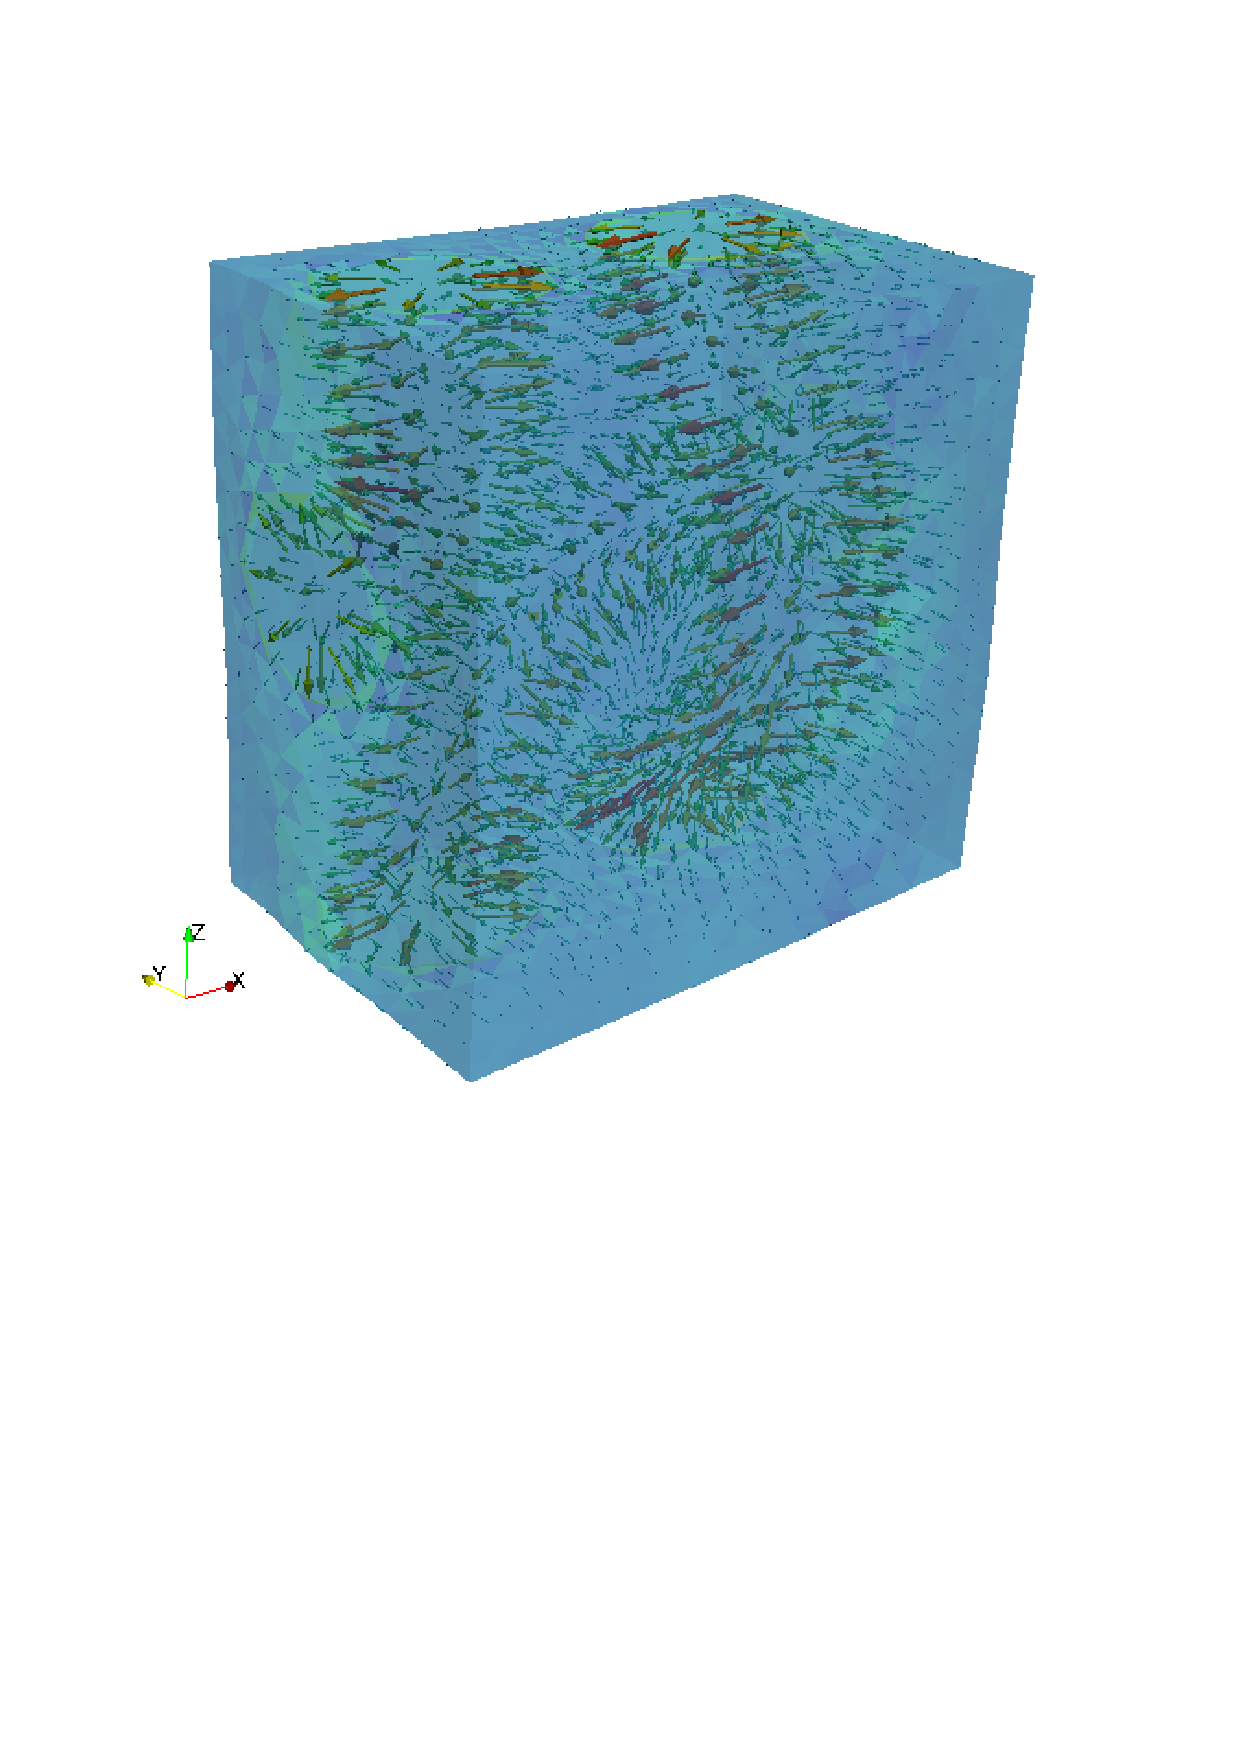
\includegraphics[width=0.5\linewidth]
        {\figDirHomPerfusion/steady_rs_00_u_M2_2}
        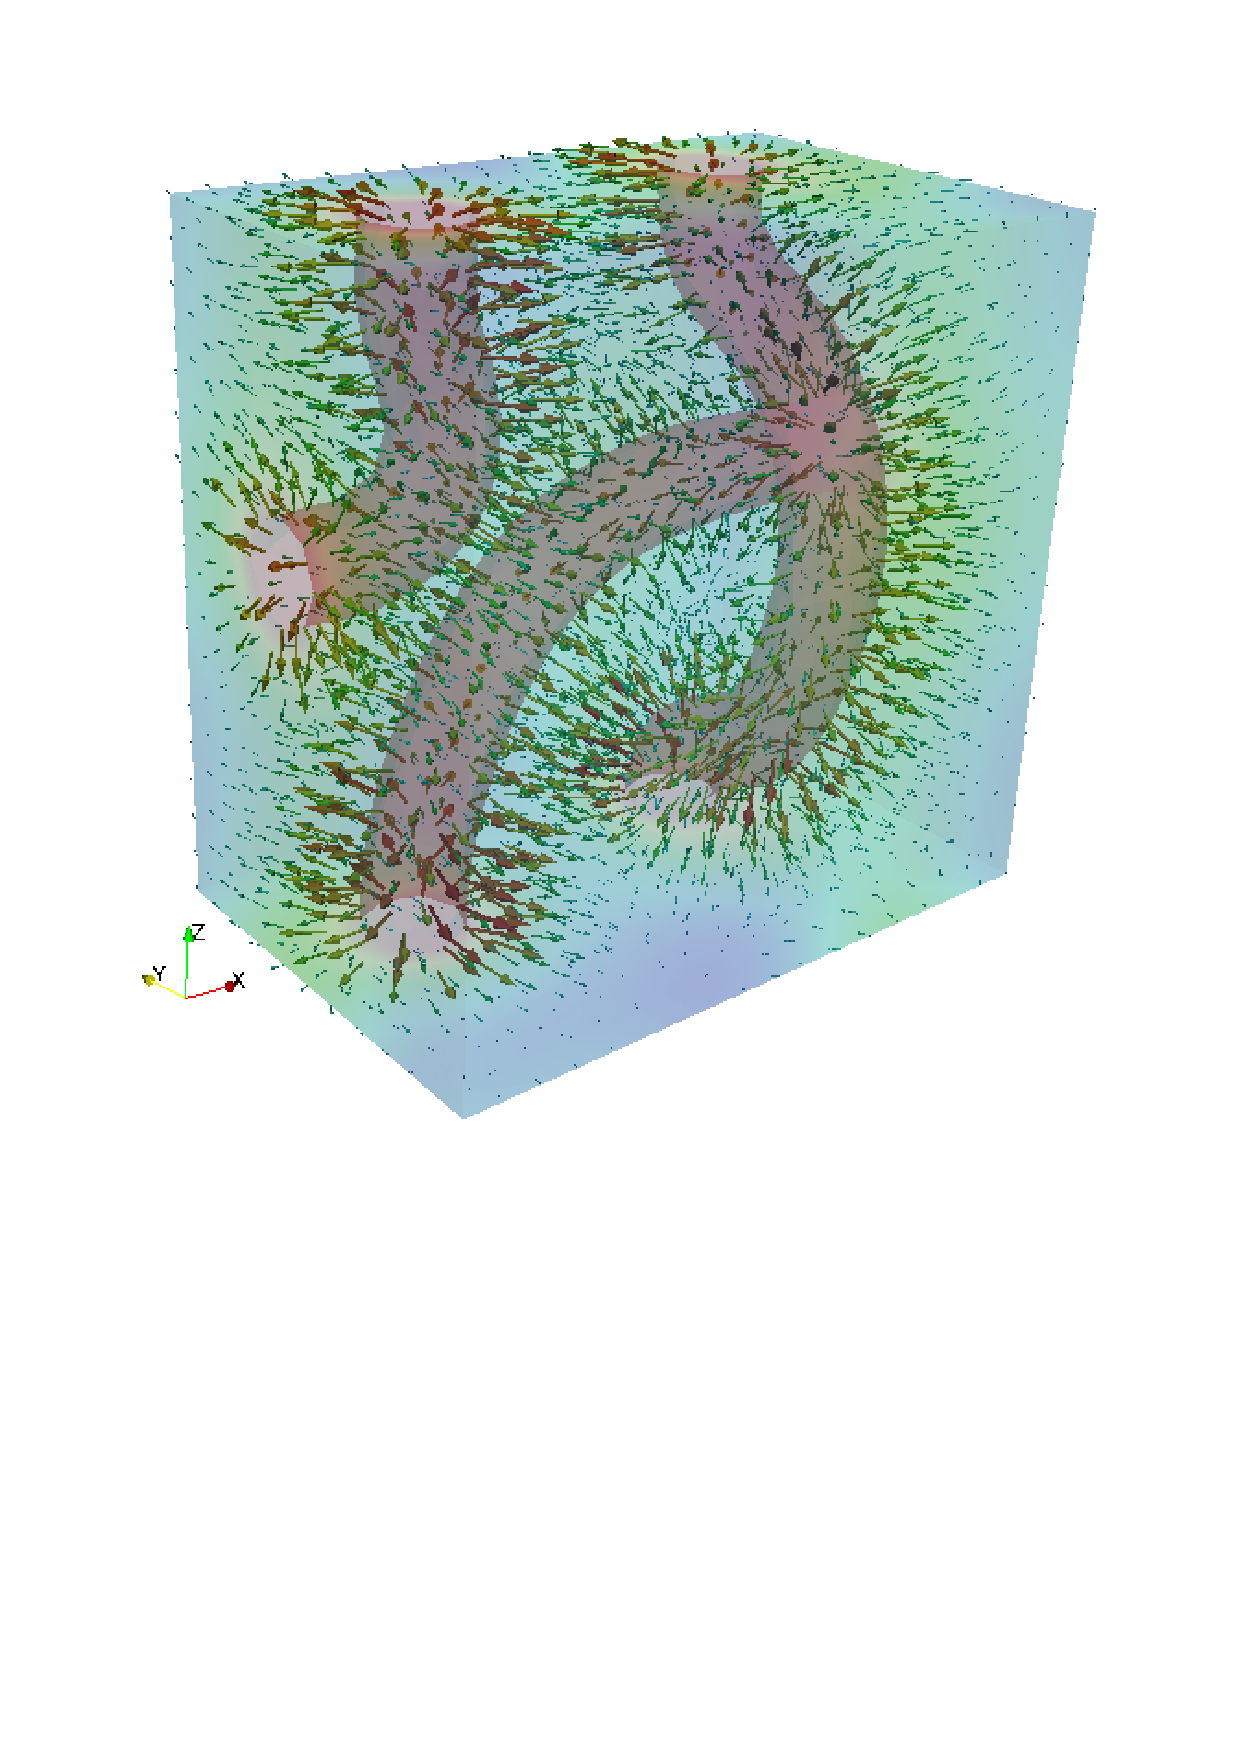
\includegraphics[width=0.5\linewidth]
        {\figDirHomPerfusion/steady_rs_00_p_M2_2}
      \end{center}
    \end{minipage}
  \end{center}
\end{frame}
